\documentclass[a4paper, 11pt]{article}
\usepackage[swedish]{babel}
\usepackage{hyperref}
\usepackage[margin=0.5in]{geometry}

\usepackage{amsmath}
\usepackage[arrowdel]{physics}

\newcommand{\V}{\mathcal{V}}
\newcommand{\ub}[1]{\vb{e}_{\vb{#1}}}
\newcommand{\cha}[1]{\delta #1}
\newcommand{\del}[3][]{\partial_{#2}^{#1}#3}
\newcommand{\mdv}[2][]{\dv[#1]{#2}{t}}
\newcommand{\integ}[5][]{\int\limits_{#2}^{#3}\dd[#1]{#4}#5}
\newcommand{\vinteg}[4]{\int\limits_{#1}^{#2}\dd{\vb{#3}}\cdot #4}
\newcommand{\tinteg}[4]{\int\limits_{#1}^{#2}\dd{\vb{#3}}\times #4}

\title{Sammanfattning av SG1218 Strömningsmekanik}
\author{Yashar Honarmandi \\ yasharh@kth.se}
\date{\today}

\begin{document}

\maketitle

\begin{abstract}
	Detta ær en sammanfattning av kursen SH1014 Modern fysik.
\end{abstract}

\pagenumbering{roman}
\thispagestyle{empty}

\newpage

\tableofcontents

\newpage

\pagenumbering{arabic}

\section{Notation}
Om inte annat specifieras, kommer alla ekvationer använda notationen som ges i denna tabellen.

\begin{table}[!h]
	\centering
	\begin{tabular}{| l | c |}
		\hline
		\textbf{Storhet} & \multicolumn{1}{|l|}{\textbf{Symbol}}\\
		Position         & $\vect{r}$ \\
		\hline
		Tid              & $t$ \\
		\hline
		Period           & $T$ \\
		\hline
		Frekvens         & $f$ \\
		\hline
		Vinkelfrekvens   & $\omega$ \\
		\hline
		Våglängd         & $\lambda$ \\
		\hline
		Vågvektor        & $\vect{k}$ \\
		\hline
		Vågtal           & $k$ \\
		\hline
		Amplitud         & $A$ \\
		\hline
		Vågfart          & $c$ \\
		\hline
	\end{tabular}
\end{table}

\section{Vektoranalys}

Vi kommer här demonstrera lite grundläggande vektoranalys för kontinua som flödar. Mer specifikt kommer vi demonstrera hur flödet påverkar hur man gör integraler i såna kontinua.

\paragraph{Hastighetsfältet}
Hastighetsfältet $\vb{u}$ är ett vektorfält som anger i vilken riktning och hur snabbt ett kontinuum flödar. Vi betecknar i bland dets komponenter som $u, v, w$.

\paragraph{Tidsändring och materiell derivata}
Betrakta ett volymselement. Om det vid en given tid befinner sig i $\vb{r}$, kommer det under en tid $\cha{t}$ förflytta sig en sträcka $\cha{\vb{r}}$. Värdet av något fält $\phi$ i det fluidelementet kommer då vara
\begin{align*}
	\phi(\vb{r} + \cha{\vb{r}}, t + \cha{t}) = \phi(\vb{r}, t) + \del{t}{\phi}\cha{t} + \del{i}{\phi}\cha{x_{i}}.
\end{align*}
Den totala tidsderivatan av $\phi$ för det givna elementet fås genom att beräkna ändringen av fältet och dela på den lilla tidsskillnaden. Vi får då
\begin{align*}
	\dv{\phi}{t} = \del{t}{\phi} + \del{i}{\phi}\frac{\cha{x_{i}}}{\cha{t}} = \del{t}{\phi} + \del{i}{\phi}u_{i} = \del{t}{\phi} + (\vb{u}\cdot\grad)\phi.
\end{align*}
Detta kallar vi för den materiella derivatan av $\phi$.

\paragraph{Tidsderivator av integraler}
Det gäller att
\begin{align*}
	\dv{t}\integ{V}{}{V}{\phi}   &= \integ{V}{}{V}{\del{t}{\phi}}, \\
	\dv{t}\integ{\V}{}{\V}{\phi} &= \integ{\V}{}{\V}{\del{t}{\phi}} + \vinteg{\mathcal{S}}{}{\mathcal{S}}{\phi\vb{u}} = \integ{\V}{}{\V}{\del{t}{\phi} + \div(\phi\vb{u})}.
\end{align*}

\section{Grundläggande koncept}

\paragraph{Syftet med reglerteknik}
Reglerteknik handlar om att kontrollera olika storheter, ofta betecknad $y$, i ett system mot något värde, ofta betecknad $r$. I tillägg till systemets egna beteende påverkas storheten vi vill reglera typiskt av en yttre störning $v$. Vi kan reglera systemet genom att tillföra en påverkan, ofta betecknad $u$.

\paragraph{Strategi}
För att förstå systemet, tar vi först fram en modell som beskriver det. Ur denna modellen fås typiskt en differentialekvation. Denna löser vi med Laplacetransform över tid.

\paragraph{Överförningsfungktionen}
För linjära system fås en lösning i Laplacerummet på formen $Y(s) = G(s)U(s)$, där $U$ är Laplacetransformen av $u$. Funktionen $G$ är överförningsfunktionen. Notera att denna lösningsformen typiskt beror på att alla initialvärden är $0$.

\paragraph{Poler}
Ett systems poler är rötterna till nämnarpolynomet (som typiskt finns) i överförningsfunktionen.

\paragraph{Stabilitet}
Ett system är stabilt om det tenderar mot ett visst läge efter lång tid. Systemets stabilitet är typiskt kopplad med dets poler. Detta kan man se i enkla fall, till exempel vanliga linjära ordinära differentialekvationer. Här är systemet stabilt om det inte finns några poler i högre halvplan, och avståndet längs med reella axeln anger hur snabbt lösningen tenderar mot det stabila läget.

\paragraph{Nollställen}
Ett systems nollställen är rötterna till täljarpolynomet (som typiskt finns) hos överförningsfunktioner. Eftersom vi är intresserade av att styra $y$, är det viktigt hur vi ska välja $u$ för att få det. Därmed är $\frac{1}{G}$ en viktig storhet, och nollställen kan därmed orsaka reglerproblem som är svårlösta.

\paragraph{Impulssvar}
Om lösningen för $Y$ är på formen $Y = GU$, är lösningen för $y$ på formen
\begin{align*}
	y(t) = \integ{0}{t}{\tau}{g(\tau)u(t - \tau)}.
\end{align*}
$g$ kallas för impulssvaret.

\paragraph{Blockschema}
Ett blockschema är ett systematisk sätt att rita reglerade system på. För att förstå hur man läser dem, betrakta figur \ref{fig:basic_block}.
\begin{figure}[!ht]
	\centering
	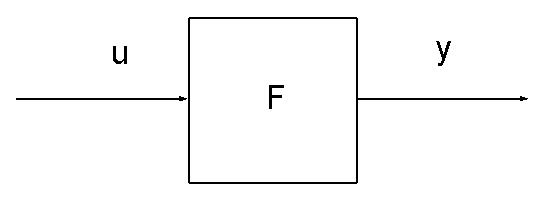
\includegraphics[width = 0.5\textwidth]{./Images/basic_block.eps}
	\caption{Illustration av ett enkelt blockschema.}
	\label{fig:basic_block}
\end{figure}

Med denna figuren menas att $Y(s) = F(s)U(s)$.

\paragraph{Rotort}
En rotort är en plott av ett systems poler som funktion av någon parameter. Den är typiskt uppdelad i grenar, som är kurvor i planet som är parametriserade av parametervärdet. Polerna som motsvarar parametervärdet $0$ är rotortens startpunkter, och polarna motsvarande parametervärdet $\infty$ är rotortens ändpunkter. Om rotorten närmar sig kurvor, är dessa rotortens asymptoter.

\section{Lösningar av Navier-Stokes' ekvation för newtonska fluider}

Detta är lösningar av Navier-Stokes' ekvation för newtonska fluider i vissa specifika geometrier.

\paragraph{Couetteströmning}
Betrakta en fluid mellan två plattor. Fluiden har kinematisk viskositet $\nu$, täthet $\rho$, konstant tryck $p$ och befinner sig långt från in- och utlopp (vi säjer att strömningen är fullt utbildad). Plattorna är på ett avstånd $h$ i $y$-riktning. Ena plattan är fäst, och andra plattan rör sig med en hastighet $U$ i $x$-riktning. Vi vill nu bestämma stationära hastighetsfältet, volymsflödet per enhet längd i $z$-riktning och spänningen på de två plattorna.

Vi noterar först att problemet är symmetriskt i både $x$ och $z$. Eftersom det inte finns något som driver flöde i $z$-riktning, måste $u_{z} = 0$. Då ger inkompressibilitetsvillkoret att $u_{y}$ är konstant och lika med $0$ för att uppfylla randvillkoret. Det som återstår av Navier-Stokes' ekvation är
\begin{align*}
	\laplacian{u_{x}} = \del[2]{y}{u_{x}} = 0,
\end{align*}
och slutligen
\begin{align*}
	u_{x} = U\frac{y}{h}.
\end{align*}

Volymsflödet per längdenhet ges av
\begin{align*}
	\Phi = \frac{1}{l}\vinteg{x = c}{}{S}{\vb{u}} = \frac{1}{l}\integ{0}{l}{z}{\integ{0}{h}{y}{U\frac{y}{h}}} = \frac{1}{2}Uh.
\end{align*}

För att hitta spänningarna längsmed ytorna, konstaterar vi först att ytorna har normalvektor $n_{i} = \pm\delta_{i2}$. Ytspänningarna ges då av
\begin{align*}
	\tau_{ij}n_{j} = \pm\tau_{i2} = \pm\mu(\del{i}{u_{2}} + \del{2}{u_{i}}).
\end{align*}
Den enda nollskilda kraftkomponenten är den första, och ges av
\begin{align*}
	f_{1} = \tau_{1j}n_{j} = \pm\mu\frac{U}{h} = \pm\frac{\rho\nu U}{h}.
\end{align*}

\paragraph{Poiseuille-strömning}
Betrakta en fluid mellan två plattor. Fluiden har kinematisk viskositet $\nu$, täthet $\rho$, tryck $p$ med konstant gradient $-K\ub{x}$ och strömningen är stationär och fullt utbildad. Plattorna är båda fästa på ett avstånd $h$ i $y$-riktning. Vi vill nu bestämma stationära hastighetsfältet, volymsflödet per längdenhet i $z$-riktning och spänningen på de två plattorna.

På samma sätt som för Couetteströmning fås $u_{y} = u_{z} = 0$ och symmetri i $x$ och $z$. Navier-Stokesä ekvation ger då
\begin{align*}
	\nu\laplacian{u_{x}} = \nu\del[2]{y}{u_{x}} = \frac{1}{\rho}\ub{x}\del{x}{p} = -\frac{K}{\rho},\ \del[2]{y}{u_{x}} = -\frac{K}{\mu}.
\end{align*}
Detta har lösning
\begin{align*}
	u_{x} = \frac{1}{2}\frac{Kh^{2}}{\mu}\left(\frac{y}{h} - \left(\frac{y}{h}\right)^{2}\right).
\end{align*}

Volymsflödet per längdenhet ges av
\begin{align*}
	\Phi &= \frac{1}{l}\vinteg{x = c}{}{S}{\vb{u}} \\
	     &= \frac{1}{l}\integ{0}{l}{z}{\integ{0}{h}{y}{\frac{1}{2}\frac{Kh^{2}}{\mu}\left(\frac{y}{h} - \left(\frac{y}{h}\right)^{2}\right)}} \\
	     &= \frac{1}{2}\frac{Kh^{3}}{\mu}\integ{0}{1}{u}{(u - u^{2})} \\
	     &= \frac{1}{12}\frac{Kh^{3}}{\mu}.
\end{align*}

Normalvektorn ges på samma sätt som innan, och vi får
\begin{align*}
	\tau_{ij}n_{j} = \pm\mu(\del{i}{u_{2}} + \del{2}{u_{i}}).
\end{align*}
Enda nollskilda komponenten är
\begin{align*}
	f_{1} = \pm\frac{1}{2}Kh\left(1 - 2\frac{y}{h}\right).
\end{align*}
Denna är lika med $\frac{1}{2}Kh$ på båda ytorna.

\paragraph{Stokes' första problem}
Betrakta en newtonsk fluid med kinematisk viskositet $\nu$ och täthet $\rho$ i det halvoändliga rummet $y > 0$. Vid randen börjar en platta röra sig med hastighet $U$ i $x$-riktningen vid $t = 0$. Vi vill nu bestämma hastighetsfältet.

Systemet är symmetriskt i $xz$-planet, och inkompressibiliteten ger då $\del{y}{u_{y}} = 0$. För att uppfylla randvillkoret måste då $u_{y} = 0$. Återigen finns det inget som driver flöde i $z$-riktning, så $u_{z} = 0$. Navier-Stokes' ekvation ger då
\begin{align*}
	\del{t}{u_{x}} = -\frac{1}{\rho}\del{x}{p} + \nu\laplacian{u_{x}}.
\end{align*}
Återigen använder vi symmetrin för att skriva detta som
\begin{align*}
	\del{t}{u_{x}} = \nu\del[2]{y}{u_{x}}.
\end{align*}
Vi kommer lösa detta med en likformighetsansats med den dimensionslösa variabeln $\eta = \frac{y}{\sqrt{\nu t}}$ på formen
\begin{align*}
	u_{x} = Uf(\eta).
\end{align*}
Jag borde lösa klart det här någon gång.

\end{document}
